\chapter{Ácidos, bases e pH}\label{ch:g9:acids-bases-ph}

Numa prateleira da cozinha estão um limão, uma garrafa de vinagre, uma
barra de sabão e uma caixa de bicarbonato de sódio; debaixo da pia, um
frasco de desentupidor com um rótulo de advertência preto e vermelho.
Alguns desses produtos têm gosto azedo, outros são escorregadios ao
toque, outros podem queimar a pele. Uma única escala, numerada de 0 a
14, classifica todos eles --- e a mesma escala é usada para as piscinas,
a terra do jardim, o sangue e os oceanos.

\begin{recall}
Os \omterm{def:g9:ions:ion}{íons} são \omterm{def:g7:atoms-and-molecules:atom}{átomos} ou grupos de \omterm{def:g7:atoms-and-molecules:atom}{átomos} com carga; um \omterm{def:g9:ions:ion}{cátion} como o
\ce{Na+} é positivo, um \omterm{def:g9:ions:ion}{ânion} como o \ce{Cl-} ou o \ce{OH-} é negativo.
As soluções iônicas contêm \omterm{def:g9:ions:ion}{íons} marcados com (aq), que se movem
livremente (\cref{ch:g9:ions}).
\end{recall}

\begin{omfigure}
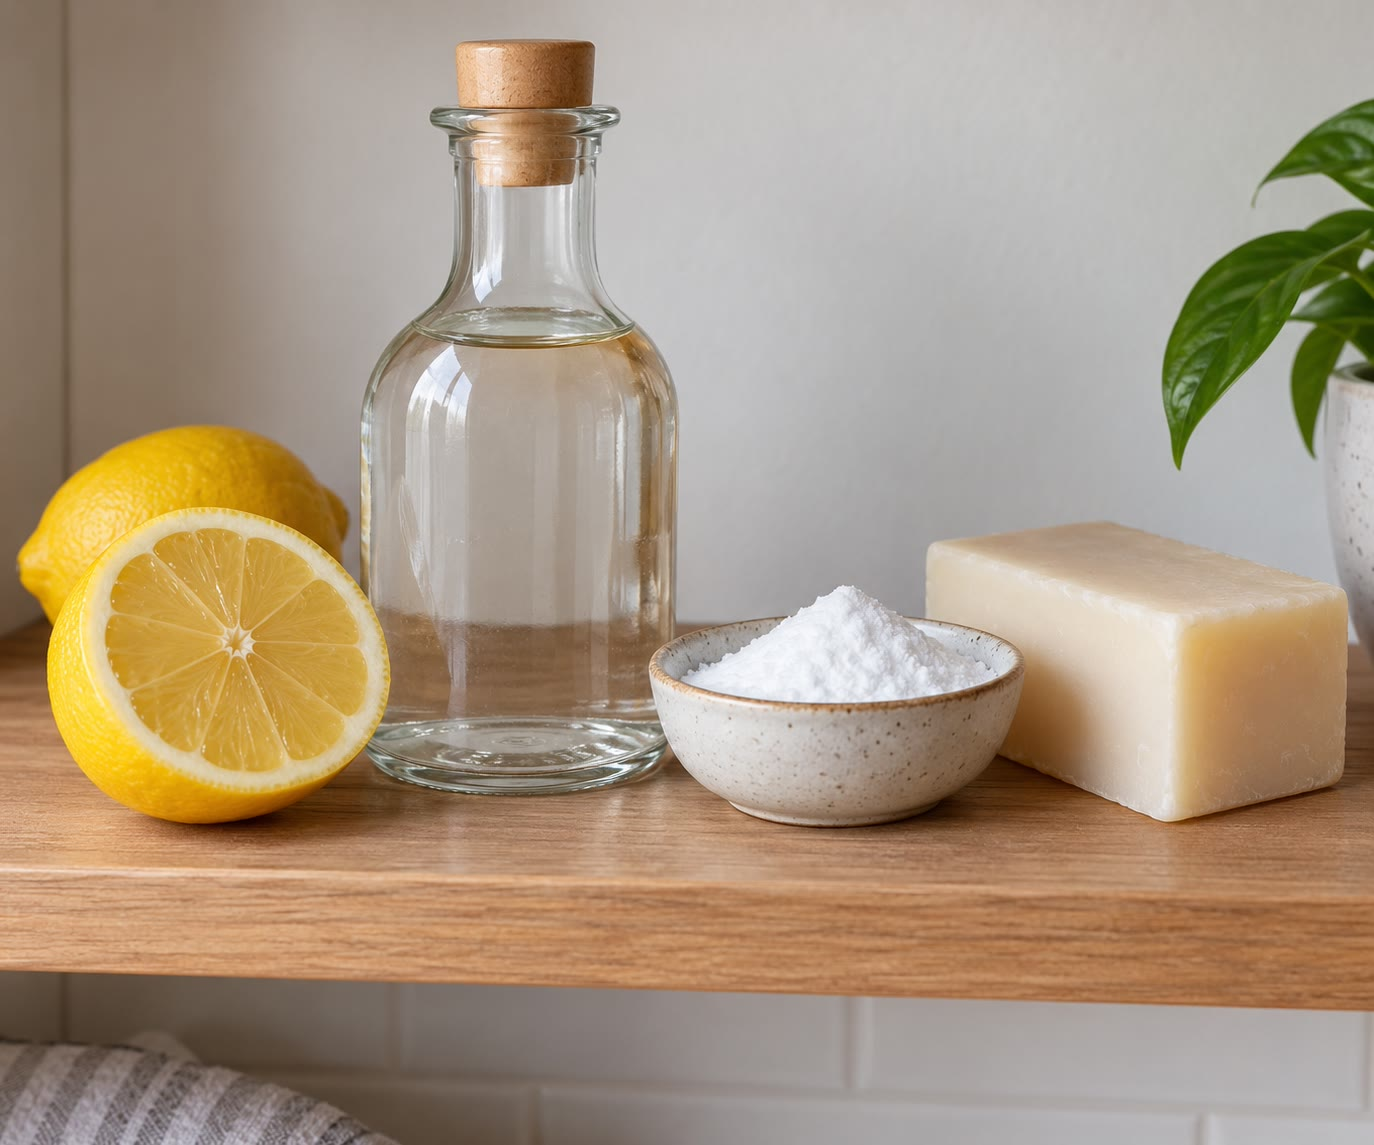
\includegraphics[width=0.55\linewidth]{images/book1/ai/g9-kitchen-shelf.jpg}

{\small Limão, vinagre, sabão e bicarbonato de sódio: ácidos e bases na
cozinha.}
\end{omfigure}

\section{Soluções ácidas, básicas e neutras}

\begin{definition}[Soluções ácidas, básicas e neutras]\label{def:g9:acids-bases-ph:acidic}
Toda \omterm{def:g6:solutions-and-solubility:solute}{solução aquosa} contém \omterm{def:g9:ions:ion}{íons} hidrogênio \ce{H+(aq)} e \omterm{def:g9:ions:ion}{íons} hidróxido
\ce{OH-(aq)}. Uma solução é uma \emph{solução ácida}\index{solucao acida@solução ácida}
quando contém mais \omterm{def:g9:ions:ion}{íons} \ce{H+} do que \omterm{def:g9:ions:ion}{íons} \ce{OH-}, uma
\emph{solução básica}\index{solucao basica@solução básica} quando contém mais \omterm{def:g9:ions:ion}{íons}
\ce{OH-} do que \omterm{def:g9:ions:ion}{íons} \ce{H+}, e uma \emph{solução
neutra}\index{solucao neutra@solução neutra} quando contém tantos de um quanto do outro.
\end{definition}

\begin{example}[Três soluções]\label{ex:g9:acids-bases-ph:three}
O ácido clorídrico é uma \omterm{def:g9:acids-bases-ph:acidic}{solução ácida}: ele contém \omterm{def:g9:ions:ion}{íons} \ce{H+(aq)} e
\ce{Cl-(aq)}, com pouquíssimos \ce{OH-}. Uma solução de hidróxido de
sódio é básica: \ce{Na+(aq)} e \ce{OH-(aq)}, com pouquíssimos \ce{H+}.
A água pura e a água salgada são neutras.
\end{example}

\section{A escala de pH}

\begin{definition}[pH]\label{def:g9:acids-bases-ph:ph}
O \emph{pH}\index{pH} de uma \omterm{def:g6:solutions-and-solubility:solute}{solução aquosa} é um número, em geral entre 0
e 14, que diz quanto ela é ácida ou básica: a \qty{25}{\celsius}, uma
\omterm{def:g9:acids-bases-ph:acidic}{solução neutra} tem pH 7, uma \omterm{def:g9:acids-bases-ph:acidic}{solução ácida} tem pH menor que 7, uma
\omterm{def:g9:acids-bases-ph:acidic}{solução básica} tem pH maior que 7. Quanto mais \omterm{def:g9:ions:ion}{íons} \ce{H+} uma solução
contém, menor é o seu pH.
\end{definition}

\begin{omfigure}
\begin{tikzpicture}[font=\small, x=0.95cm]
  \foreach \k in {0,...,13} {
    \pgfmathtruncatemacro\rr{2.2*max(0,100-14.3*\k)+30}
    \pgfmathtruncatemacro\gg{1.8*(\k<7 ? 30+10*\k : 100-8*(\k-7))+40}
    \pgfmathtruncatemacro\bb{2.2*max(0,14.3*(\k-6))+30}
    \definecolor{phc}{RGB}{\rr,\gg,\bb}
    \fill[phc] (\k,0) rectangle ++(1,0.6);
  }
  \foreach \k in {0,...,14} \node[anchor=north, font=\footnotesize] at (\k,-0.02) {\k};
  \draw[black!60] (0,0) rectangle (14,0.6);
  \node[anchor=south] at (3.5,0.65) {ácida};
  \node[anchor=south] at (7,0.65) {neutra};
  \node[anchor=south] at (10.5,0.65) {básica};
  % ledger: ph:HCl-1M, ph:gastric, ph:lime, ph:wine, ph:coffee, ph:pure-water, ph:seawater, ph:milk-magnesia, ph:ammonia, ph:NaOH-1M
  \foreach \x/\lab/\lev/\anc in {0/{ácido\\ clorídrico (1 M)}/1/north, 1.5/{suco\\ gástrico}/3/north east,
      2/{suco de\\ limão}/2/north west, 3.5/{vinho}/1/north, 5/{café}/2/north, 7/{água\\ pura}/3/north,
      8.1/{água do\\ mar}/1/north, 10.5/{leite de\\ magnésia}/3/north, 12/{amoníaco\\ doméstico}/1/north,
      14/{hidróxido de sódio\\ (1 M)}/2/north east} {
    \draw[black!55] (\x,-0.45) -- (\x,-0.45-0.8*\lev);
    \node[anchor=\anc, font=\footnotesize, align=center, inner sep=2pt] at (\x,-0.45-0.8*\lev) {\lab};
  }
\end{tikzpicture}

{\small A escala de \omterm{def:g9:acids-bases-ph:ph}{pH}, com o \omterm{def:g9:acids-bases-ph:ph}{pH} de algumas soluções comuns.}
\end{omfigure}

\begin{definition}[Papel indicador e pHmetro]\label{def:g9:acids-bases-ph:ph-paper}
O \emph{papel indicador de pH}\index{papel indicador de pH} é uma tira
de papel impregnada de uma \omterm{def:g6:pure-substances-and-mixtures:mixture}{mistura} de corantes que assume uma cor
diferente em cada \omterm{def:g9:acids-bases-ph:ph}{pH}; uma gota da solução é posta sobre ele e a cor é
comparada com uma tabela impressa na caixa. Um
\emph{pHmetro}\index{pHmetro} mede o \omterm{def:g9:acids-bases-ph:ph}{pH} com um eletrodo de vidro
mergulhado na solução e o mostra como um número, com uma ou duas casas
decimais.
\end{definition}

\begin{method}[Medir um pH com papel indicador]\label{met:g9:acids-bases-ph:paper}
\begin{enumerate}
  \item Ponha uma tira curta de papel indicador num pratinho limpo e
        seco.
  \item Com um bastão de vidro limpo, toque a tira com uma gota da
        solução (nunca mergulhe a tira no frasco).
  \item Compare a cor imediatamente com a tabela e leia o \omterm{def:g9:acids-bases-ph:ph}{pH}, em geral
        até o número inteiro mais próximo.
\end{enumerate}
\end{method}

\begin{omfigure}
\begin{tikzpicture}[font=\small, scale=1.2]
  \pic[transform shape] at (0,0) {stirrer};
  \pic[transform shape] at (0,0.05) {beaker={0.55}{omWater!80}};
  \pic[transform shape] at (0.25,0.35) {probe};
  \pic[transform shape] at (2.6,3.4) {meter={pH}};
  \draw[black!70, line width=0.6pt] (0.25,3.45) .. controls (0.3,4.3) and (2.2,4.4)
    .. (2.2,2.95);
  \draw[<-, omProp, thick] (0.4,1.0) -- (2.0,1.3) node[right, text=black] {eletrodo de vidro};
  \draw[<-, omProp, thick] (3.35,3.4) -- (4.0,3.4) node[right, text=black] {pHmetro};
  \draw[<-, omProp, thick] (-0.6,0.6) -- (-1.6,0.9) node[left, text=black] {solução};
\end{tikzpicture}

{\small Medir um \omterm{def:g9:acids-bases-ph:ph}{pH} com um \omterm{def:g9:acids-bases-ph:ph-paper}{pHmetro}: o eletrodo de vidro fica mergulhado
na solução, que é agitada devagar.}
\end{omfigure}

\section{Diluir um ácido}

\begin{proposition}[Diluir aproxima o pH de 7]\label{prop:g9:acids-bases-ph:dilution}
Acrescentar água a uma \omterm{def:g9:acids-bases-ph:acidic}{solução ácida} espalha os seus \omterm{def:g9:ions:ion}{íons} \ce{H+} num
volume maior: o \omterm{def:g9:acids-bases-ph:ph}{pH} sobe, em direção a 7, mas nunca passa de 7. Para um
ácido como o ácido clorídrico, diluir dez vezes aumenta o \omterm{def:g9:acids-bases-ph:ph}{pH} em cerca
de uma unidade: um volume de ácido de \omterm{def:g9:acids-bases-ph:ph}{pH} 2 mais nove volumes de água dão
uma solução de \omterm{def:g9:acids-bases-ph:ph}{pH} 3. Do mesmo modo, diluir uma \omterm{def:g9:acids-bases-ph:acidic}{solução básica} diminui o
seu \omterm{def:g9:acids-bases-ph:ph}{pH} em direção a 7.
\end{proposition}

\begin{omfigure}
\begin{tikzpicture}[font=\small, scale=1.05]
  \foreach \k/\ph/\cc in {0/2/red!38!omWater,1/3/red!24!omWater,2/4/red!12!omWater} {
    \pic[transform shape] at (\k*4.4,0) {beaker={0.55}{\cc}};
    \node[anchor=north, align=center] at (\k*4.4,-0.15) {pH \ph};
  }
  \foreach \k in {0,1} \draw[->, thick, omProp] (\k*4.4+1.1,1.0) -- (\k*4.4+3.3,1.0)
    node[midway, above, text=black, font=\footnotesize, align=center]
    {10 mL + 90 mL\\ de água};
\end{tikzpicture}

{\small Diluir um ácido dez vezes, e depois mais dez vezes: o \omterm{def:g9:acids-bases-ph:ph}{pH} passa de
2 para 3 e depois para 4 (cada béquer é um décimo da solução anterior
completado com água).}
\end{omfigure}

\begin{inthelab}[Diluir um ácido]
Para diluir um ácido, o professor sempre despeja o ácido devagar na
água, nunca a água no ácido: a \omterm{def:g6:pure-substances-and-mixtures:mixture}{mistura} libera calor, e a água despejada
sobre um ácido concentrado pode ferver na hora e espirrar ácido para
fora do recipiente.
\end{inthelab}

\section{Ácidos e bases do dia a dia}

\begin{proposition}[Ácidos e bases à nossa volta]\label{prop:g9:acids-bases-ph:everyday}
Ácidos: o suco de limão, o vinagre, o vinho, os refrigerantes, o café, o
suco gástrico do estômago. Básicos: a água do mar (levemente), o
bicarbonato de sódio dissolvido em água, o sabão, o leite de magnésia
(um remédio contra a acidez do estômago), o amoníaco doméstico, a água
sanitária, o desentupidor (muito fortemente).
\end{proposition}

\begin{example}[O pH do oceano]\label{ex:g9:acids-bases-ph:ocean}
% ledger: ph:seawater, ph:ocean-drop
O \omterm{def:g9:acids-bases-ph:ph}{pH} médio do oceano é cerca de 8.1: levemente básico. Desde o começo da
era industrial, o dióxido de carbono que \omterm{def:g2:mixing-and-dissolving:dissolve}{se dissolve} a partir do \omterm{def:g4:air-a-mixture-of-gases:air}{ar}
diminuiu o \omterm{def:g9:acids-bases-ph:ph}{pH} das águas de superfície em cerca de 0.1: os oceanos estão
ficando aos poucos menos básicos, o que prejudica os moluscos e os
corais.
\end{example}

\begin{omfigure}
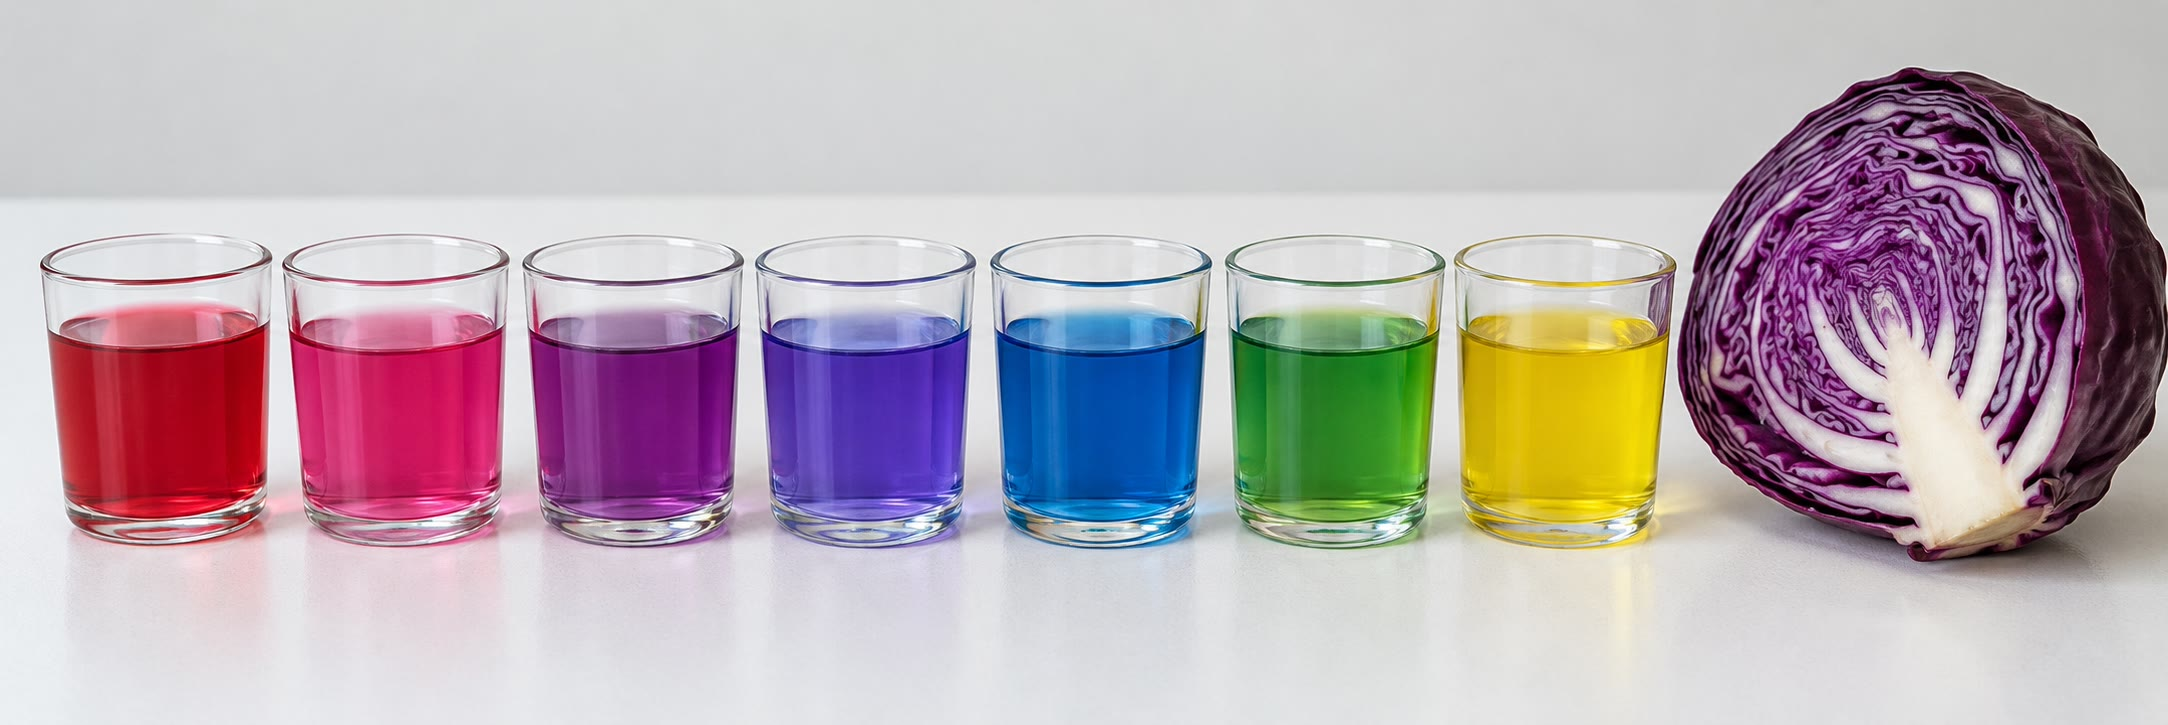
\includegraphics[width=0.55\linewidth]{images/book1/ai/g9-red-cabbage.jpg}

{\small O suco de repolho roxo, preparado por um professor, muda de cor
com o \omterm{def:g9:acids-bases-ph:ph}{pH}: vermelho nos ácidos, violeta perto do neutro, azul, verde e
depois amarelo em soluções cada vez mais básicas.}
\end{omfigure}

\section{Segurança com produtos corrosivos}

\begin{safety}{\ghs[0.85cm]{GHS05}\ghs[0.85cm]{GHS07}}
% ledger: ghs:HCl, ghs:NaOH
O ácido clorídrico concentrado e o hidróxido de sódio (a base dos
desentupidores) trazem o pictograma de corrosão GHS05: eles provocam
queimaduras graves na pele e nos olhos e atacam os metais. GHS07:
irritante. Óculos de proteção e luvas; um respingo é enxaguado na hora
com muita água.
\end{safety}

\begin{remark}[Nunca misture produtos de limpeza]\label{rem:g9:acids-bases-ph:mix}
Os produtos ácidos e básicos reagem entre si, às vezes violentamente, e
algumas \omterm{def:g6:pure-substances-and-mixtures:mixture}{misturas} liberam gases tóxicos: a água sanitária \omterm{def:g2:mixing-and-dissolving:mix}{misturada} com
um removedor de calcário ácido libera cloro. Os produtos de limpeza
nunca são \omterm{def:g2:mixing-and-dissolving:mix}{misturados}.
\end{remark}

\section{Exercícios}

\begin{exercise}[$\star$]\label{exo:g9:acids-bases-ph:1}
Ácida, básica ou neutra? Uma solução de \omterm{def:g9:acids-bases-ph:ph}{pH} 3, uma de \omterm{def:g9:acids-bases-ph:ph}{pH} 7, uma de
\omterm{def:g9:acids-bases-ph:ph}{pH} 11.
\end{exercise}

\begin{exercise}[$\star$]\label{exo:g9:acids-bases-ph:2}
Que \omterm{def:g9:ions:ion}{íons} são mais numerosos numa \omterm{def:g9:acids-bases-ph:acidic}{solução ácida}? E numa básica?
\end{exercise}

\begin{exercise}[$\star$]\label{exo:g9:acids-bases-ph:3}
Usando a escala de \omterm{def:g9:acids-bases-ph:ph}{pH} deste capítulo, ponha em ordem, da mais ácida à
mais básica: café, água do mar, suco de limão, amoníaco doméstico, água
pura.
\end{exercise}

\begin{exercise}[$\star$]\label{exo:g9:acids-bases-ph:4}
Descreva como medir o \omterm{def:g9:acids-bases-ph:ph}{pH} de uma solução com papel indicador.
\end{exercise}

\begin{exercise}[$\star\star$]\label{exo:g9:acids-bases-ph:5}
Uma solução de \omterm{def:g9:acids-bases-ph:ph}{pH} 4 é diluída dez vezes com água. Qual é, mais ou menos,
o novo \omterm{def:g9:acids-bases-ph:ph}{pH} dela? E se ela for diluída cem vezes?
\end{exercise}

\begin{exercise}[$\star\star$]\label{exo:g9:acids-bases-ph:6}
Uma \omterm{def:g9:acids-bases-ph:acidic}{solução ácida} pode ficar básica com o acréscimo de água? Explique.
\end{exercise}

\begin{exercise}[$\star\star$]\label{exo:g9:acids-bases-ph:7}
Por que se deve despejar o ácido na água, e não o contrário?
\end{exercise}

\begin{exercise}[$\star\star$]\label{exo:g9:acids-bases-ph:8}
Um frasco traz o pictograma GHS05. O que ele significa? Dê duas
precauções.
\end{exercise}

\begin{exercise}[$\star\star$]\label{exo:g9:acids-bases-ph:9}
Quantas diluições de dez vezes são necessárias para levar um ácido de
\omterm{def:g9:acids-bases-ph:ph}{pH} 1 a \omterm{def:g9:acids-bases-ph:ph}{pH} 4? Que diluição total é essa?
\end{exercise}

\begin{exercise}[$\star\star$]\label{exo:g9:acids-bases-ph:10}
O leite de magnésia é tomado contra a acidez do estômago. Usando a
escala de \omterm{def:g9:acids-bases-ph:ph}{pH}, explique por quê.
\end{exercise}

\begin{exercise}[$\star\star\star$]\label{exo:g9:acids-bases-ph:11}
O \omterm{def:g9:acids-bases-ph:ph}{pH} do oceano caiu cerca de 0.1 desde a era industrial. O oceano é
ácido hoje? Em que sentido ele está mudando, e por quê?
\end{exercise}

\begin{exercise}[$\star\star\star$]\label{exo:g9:acids-bases-ph:12}
Um aluno mede o \omterm{def:g9:acids-bases-ph:ph}{pH} do mesmo vinagre com papel indicador (3) e com um
\omterm{def:g9:acids-bases-ph:ph-paper}{pHmetro} (2.6). Explique por que os dois resultados são diferentes e
qual é mais preciso.
\end{exercise}

\section{Problema: o ácido derramado}

\begin{problem}[{Problema de fim de semana --- um litro de ácido
derramado na pia de um laboratório, e por que diluí-lo não é a solução}]
\label{pb:g9:acids-bases-ph:1}
Um frasco com \qty{1}{L} de ácido clorídrico diluído, de \omterm{def:g9:acids-bases-ph:ph}{pH} 2, quebra na
pia de um laboratório. O esgoto não pode receber nenhuma solução de \omterm{def:g9:acids-bases-ph:ph}{pH}
menor que 5. Use a regra deste capítulo: para esse ácido, cada diluição
de dez vezes aumenta o \omterm{def:g9:acids-bases-ph:ph}{pH} em uma unidade.

\medskip
\noindent\textbf{Parte I --- O ácido.}
\begin{enumerate}
  \item A solução é ácida, neutra ou básica? Que \omterm{def:g9:ions:ion}{íons} ela contém em maior
        quantidade?
  \item Que pictograma o frasco deve trazer, e por quê?
  \item O professor mede o \omterm{def:g9:acids-bases-ph:ph}{pH} com um \omterm{def:g9:acids-bases-ph:ph-paper}{pHmetro} em vez de papel indicador.
        Dê uma vantagem.
  \item Quantas vezes mais \omterm{def:g9:ions:ion}{íons} \ce{H+} há num litro de \omterm{def:g9:acids-bases-ph:ph}{pH} 2 do que num
        litro de \omterm{def:g9:acids-bases-ph:ph}{pH} 3 do mesmo ácido?
\end{enumerate}

\medskip
\noindent\textbf{Parte II --- Diluir.}
\begin{enumerate}[resume]
  \item Que volume de solução se obtém diluindo dez vezes o litro de
        ácido? Qual é o \omterm{def:g9:acids-bases-ph:ph}{pH} dela?
  \item Quantas diluições de dez vezes são necessárias para chegar a
        \omterm{def:g9:acids-bases-ph:ph}{pH} 5?
  \item Que volume total de solução isso daria?
  \item Alguma quantidade de água poderia deixar a \omterm{def:g9:acids-bases-ph:acidic}{solução básica}?
        Explique.
\end{enumerate}

\medskip
\noindent\textbf{Parte III --- Um jeito melhor.}
O professor acrescenta, em vez disso, pouco a pouco, uma solução de uma
base até que o papel indicador mostre 7: os \omterm{def:g9:ions:ion}{íons} \ce{H+} do ácido reagem
com os \omterm{def:g9:ions:ion}{íons} \ce{OH-} da base.
\begin{enumerate}[resume]
  \item Escreva a equação da reação entre os \omterm{def:g9:ions:ion}{íons} \ce{H+} e \ce{OH-}.
  \item Por que isso é melhor do que diluir?
  \item Dê o nome de um produto básico do dia a dia que poderia ser usado
        numa cozinha para limpar um pequeno derramamento de vinagre.
  \item Calcule o volume de água que teria de ser acrescentado ao litro
        de ácido para levá-lo a \omterm{def:g9:acids-bases-ph:ph}{pH} 5.
\end{enumerate}
\end{problem}
